\begin{figure}[t]
\centering
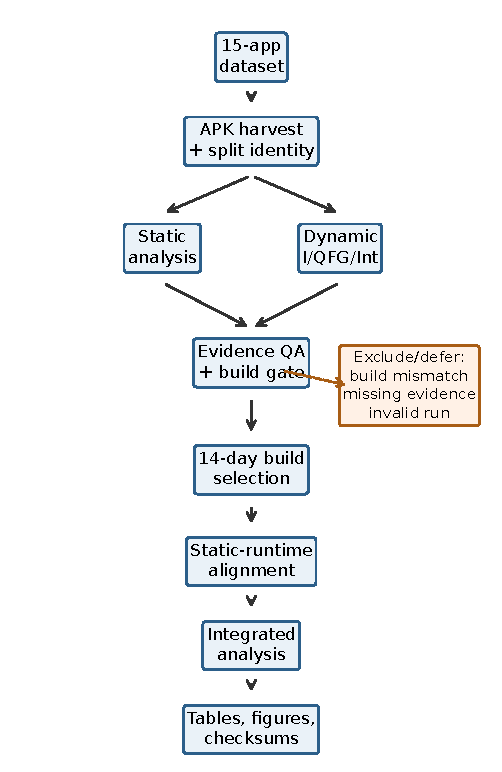
\includegraphics[width=\columnwidth]{figures/fig1_study_pipeline.pdf}
\caption{Static and runtime evidence pipeline used to assemble build-backed app bundles.}
\label{fig:fig1_study_pipeline}
\end{figure}

\begin{figure}[t]
\centering
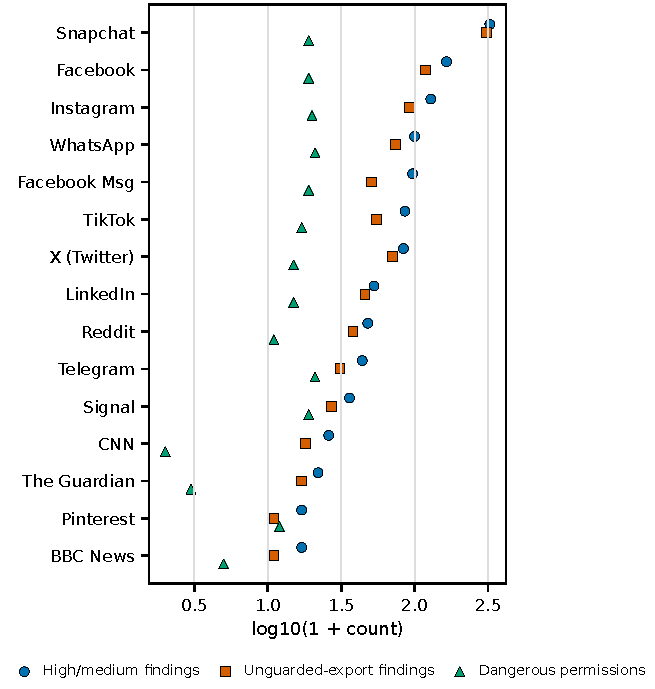
\includegraphics[width=\columnwidth]{figures/fig2_static_exposure_heatmap.pdf}
\caption{Normalized static exposure indicators across the 15-app dataset.}
\label{fig:fig2_static_exposure_heatmap}
\end{figure}

\begin{figure}[t]
\centering
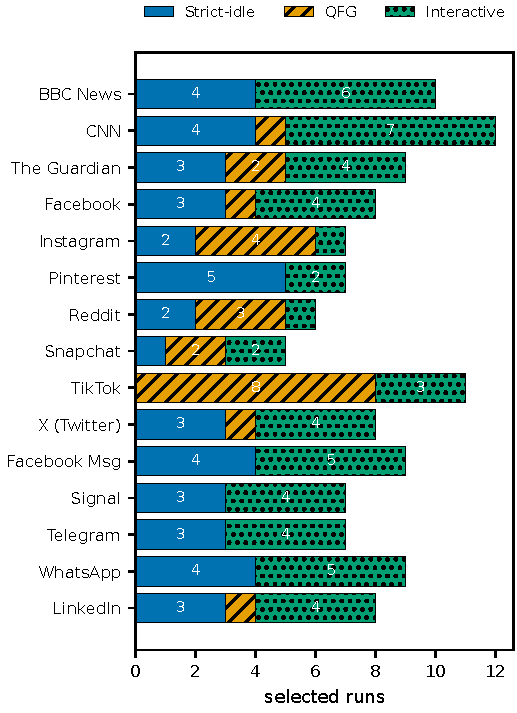
\includegraphics[width=\columnwidth]{figures/fig3_runtime_coverage_by_app.pdf}
\caption{Selected runtime evidence classes by app. QFG is reported separately from strict idle.}
\label{fig:fig3_runtime_coverage_by_app}
\end{figure}

\begin{figure}[t]
\centering
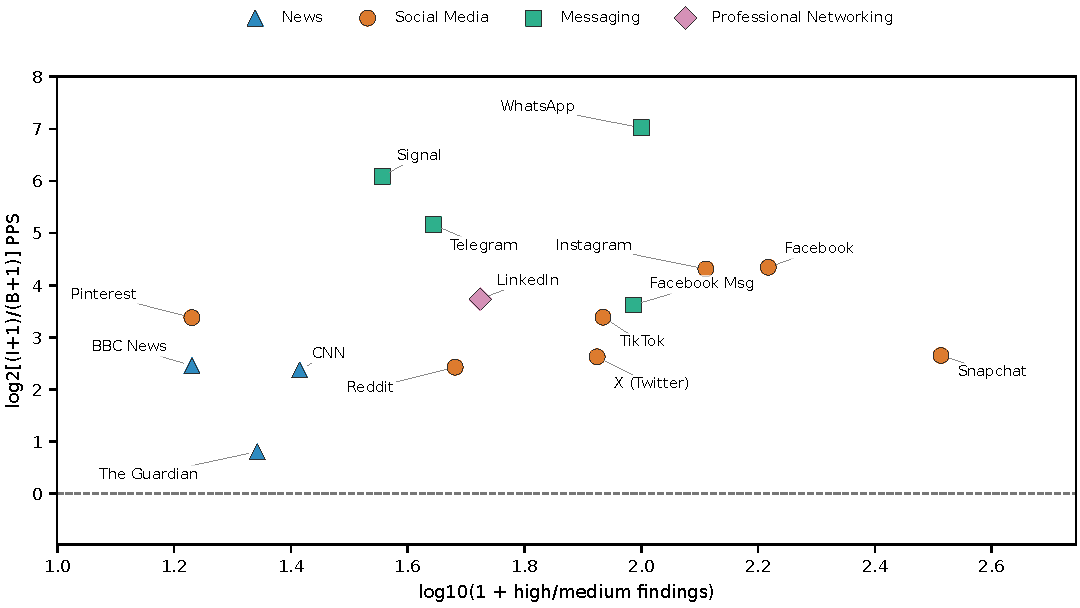
\includegraphics[width=\columnwidth]{figures/fig4_static_runtime_scatter.pdf}
\caption{High- and medium-severity static findings compared with PCAP-backed runtime evidence depth.}
\label{fig:fig4_static_runtime_scatter}
\end{figure}
